\subsection{Aantal trainingssessies}
Intu\"itie zegt dat hoe meer gelegenheden het netwerk krijgt om te trainen, hoe beter het netwerk wordt. Hier willen we kijken wat de bovengrens is en tot waar extra trainingssessies weinig invloed hebben op het netwerk.

\begin{table}[ht]
    \centering
      $\begin{array}{c||c|c |}
        \text{Aantal trainingssessies} & \text{Aantal correct} & \text{Percentage \% correct} \\ \hline
        1 & 0 & 0 \\ \hline
        100000 & 15 & 30 \\ \hline
        200000 & 36 & 72 \\ \hline
        300000 & 38 & 76 \\ \hline
        400000 & 44 & 88 \\ \hline
        500000 & 41 & 82 \\ \hline
        600000 & 42 & 84 \\ \hline
        700000 & 43 & 86 \\ \hline
        800000& 46 & 92 \\ \hline
        900000 & 45 & 90 \\ \hline
        1000000 & 43 & 86 \\ \hline
        1100000 & 48 & 96 \\ \hline
        1200000 & 46 & 92 \\ \hline
        1300000 & 48 & 96 \\ \hline
        1400000 & 46 & 92 \\ \hline
        1500000 & 46 & 92 \\ \hline
      \end{array}$
    \caption{Aantal correcte antwoorden over 50 executies met verschillende aantallen trainingssessies}
    \label{tab:training}
\end{table}

\begin{figure}[ht!]
    \centering
    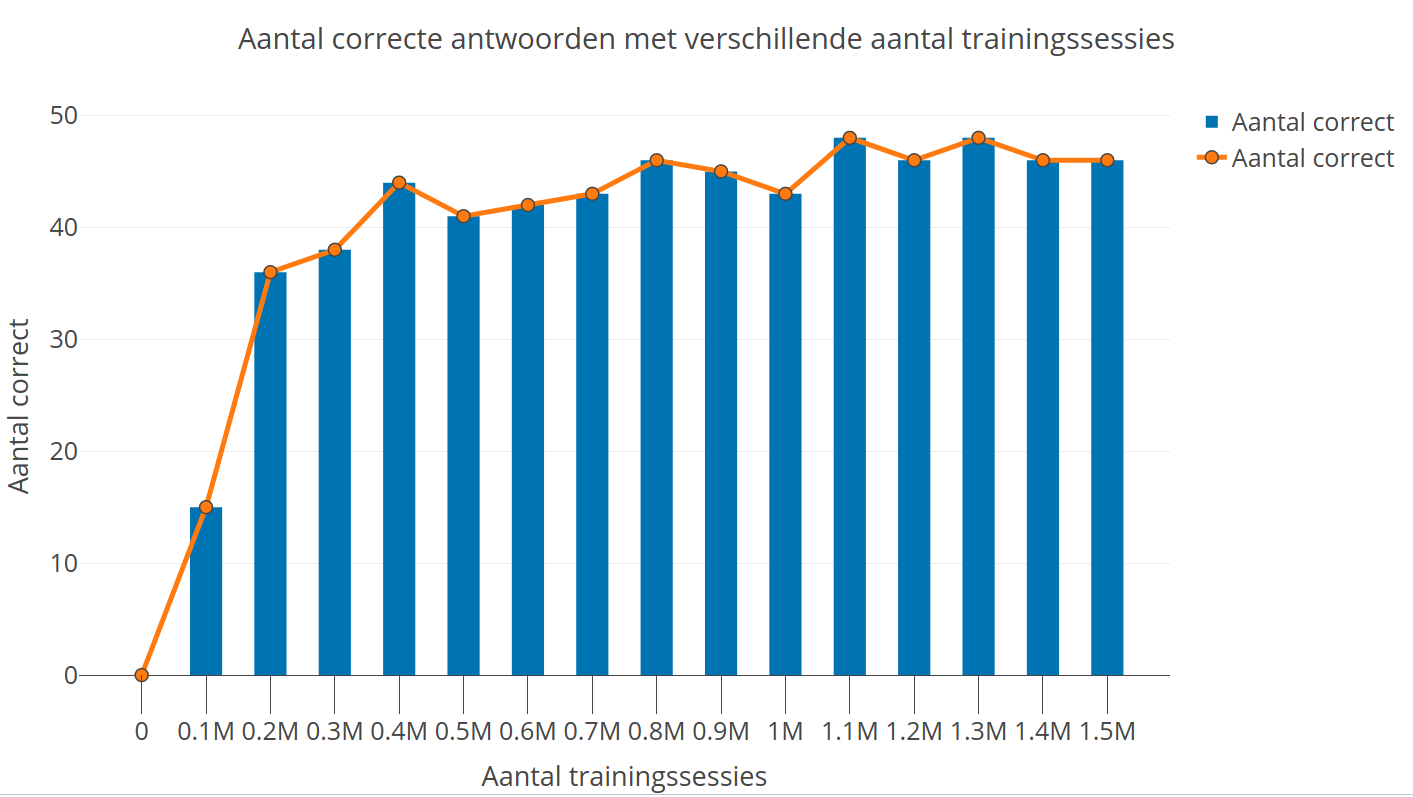
\includegraphics[scale=0.3]{graphs/training.png}
    \caption{Aantal correcte antwoorden over 50 executies met verschillende aantallen trainingssessies}
    \label{fig:training}
\end{figure}

We zien in Tabel \ref{tab:training} en Figuur \ref{fig:training} dat het netwerk inderdaad beter wordt met meer trainingssessies, zoals verwacht. De piek lijkt te zijn geraakt rond de 800000 trainingssessies, waarna er kleine verschillen zijn in opeenvolgende getallen. We kunnen zien dat er wel degelijk een limiet zit aan het aantal trainingssessies dat het netwerk kan doen, voordat het geen effect meer heeft.
